%----------------------------------------------------------------------------
\chapter{A multiprocesszoros OpenCL környezet}
%----------------------------------------------------------------------------

\section{OpenCL architektúrája}
	Az Open Computing Language (OpenCL) keretrendszer \cite{opencl}
	általános modellt, magas szintű programozási interfészt és hardware
	absztrakciót nyújt a fejlesztőknek adat- vagy feladat párhuzamos számítások gyorsítására különböző
	számítóegységen (CPU, GPU, FPGA, DSP, \ldots).
	A hárdvergyártók implementálják az OpenCL szabványt, ami által saját platformot
	hoznak létre. Egy ilyen platformon belüli eszközök alatt főként GPU-kat, de
	CPU-kat és FPGA-t \ldots is értünk.
	OpenCL keretrendszerben történő programozás során két programot kell írnunk.
	Az egyik a kernel, ami az eszközön futatott szálra fog leképeződni.
	A másik a gazda processzoron (host-on) futó host-program, ami elvégzi a
	probléma összeállítását, memória allokálást, argumentumok beállítását
	illetve a kernel meghívását az eszközön.
	A kernel futása végeztével a host-program kiolvassa az eszközből
	a kívánt eredményt.
	
	\begin{figure}[!h]
		\centering
		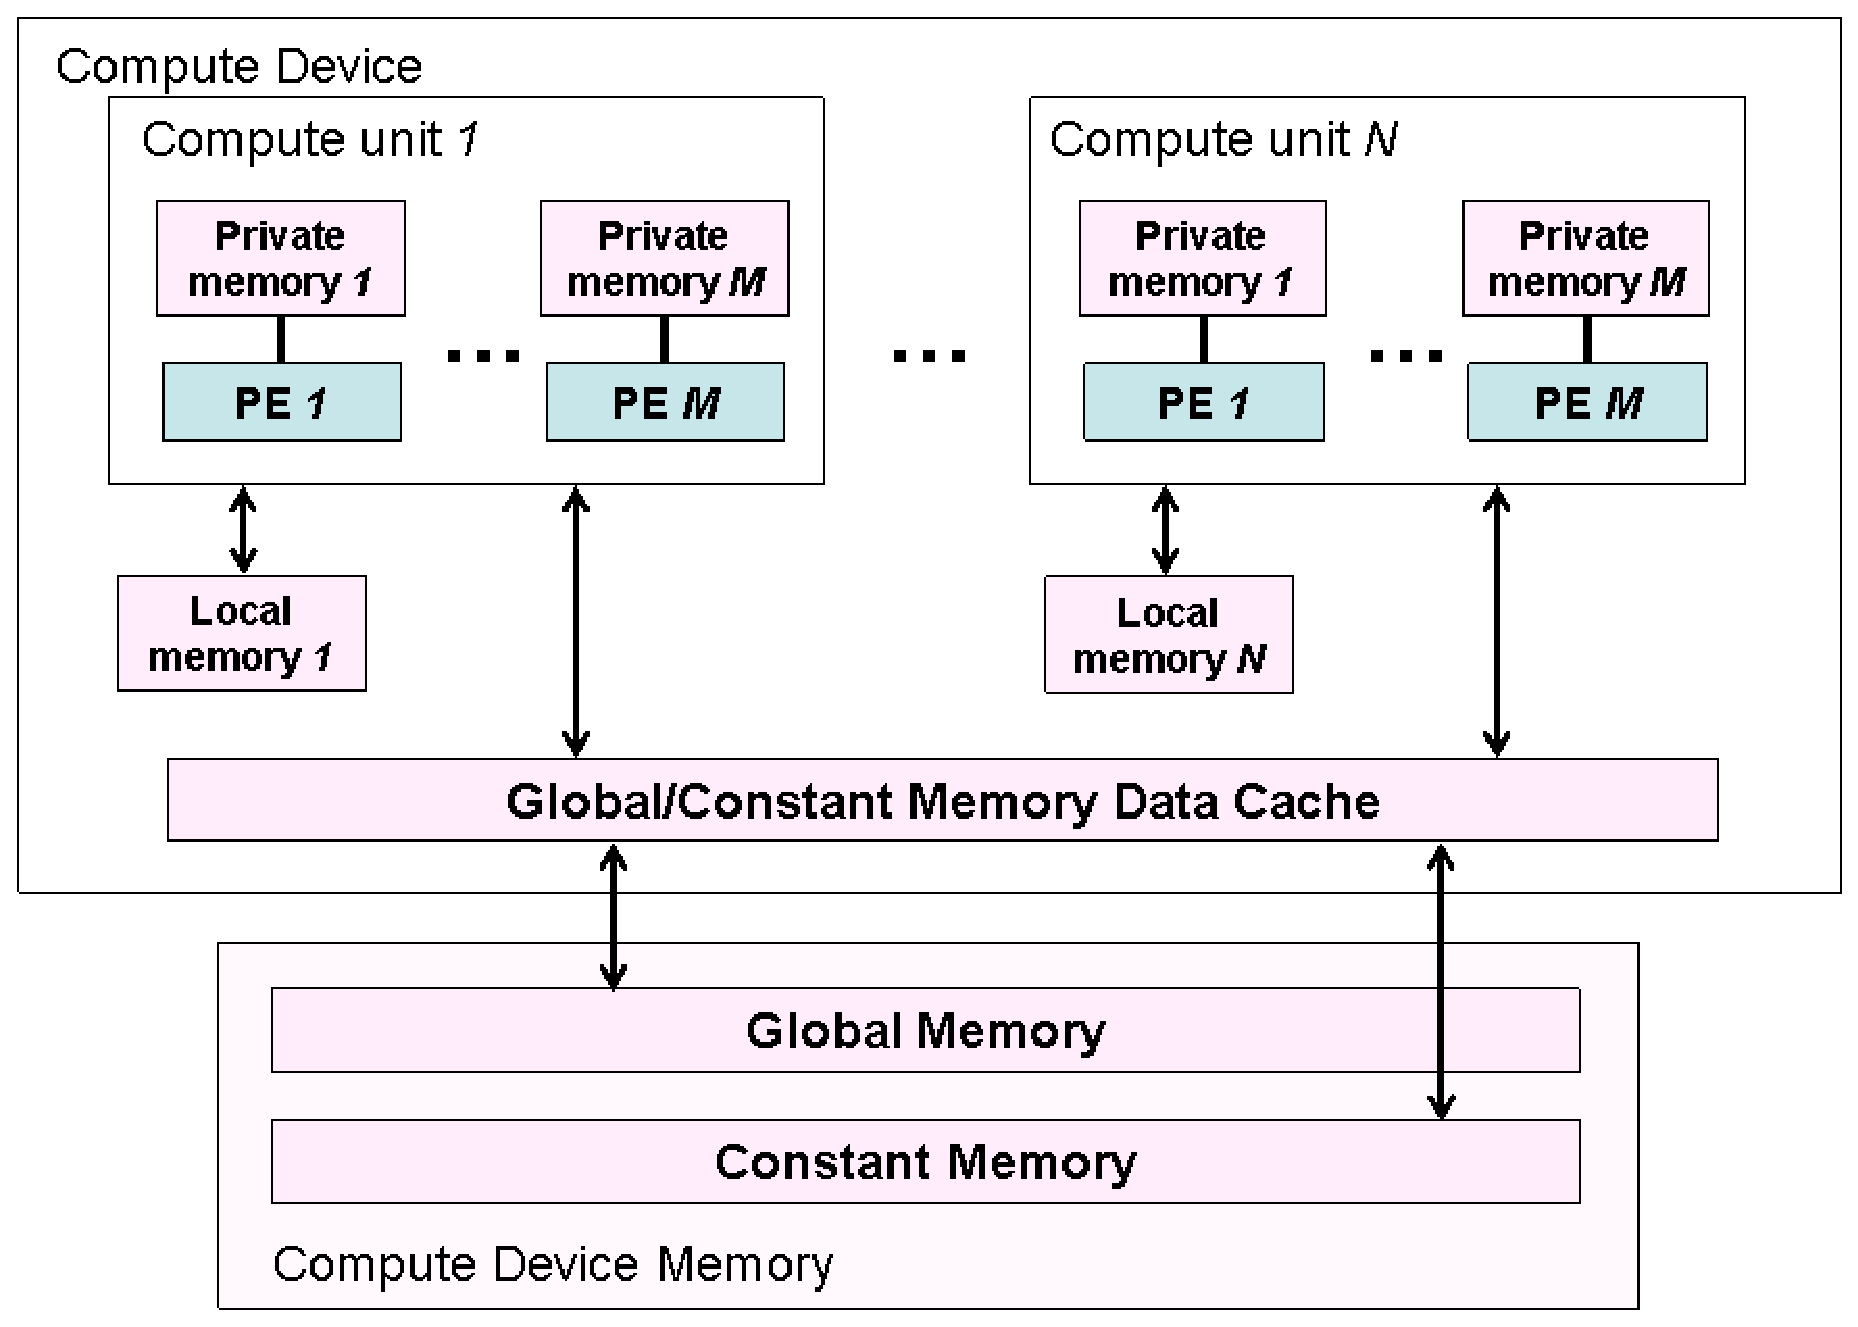
\includegraphics[width=0.6\columnwidth]{figures/eps/device.eps}
		\caption{OpenCL device architektúra \cite{opencl}} 
		\label{fig:device} 
	\end{figure}
	Az eszközök multiprocesszoros architektúrával és ezek kiszolgálására képes
	memória architektúrával rendelkeznek, amit a \ref{fig:device} ábra vázol.
	Egy eszköz több compute unit-ot (processzor-magot) tartalmaz.
	Az OpenCL négy memória szintet különböztet meg, amikre a
	következőképpen hivatkozik:
	\begin{itemize}
		\item \emph{Regiszterek:} Private memory,
		\item \emph{Chipen belüli memória (cache):} Local memory,
		\item \emph{Chipen kívüli memória:} Global memory és Constant Memory.
	\end{itemize}
	A regiszterek és lokális memória kis méretűnek és gyors elérésűnek modható, míg
	a globális memória nagynak de lassú elérésűnek.
	A memóriákra megkötésként szolgál, hogy ki allokálhat, írhat és olvashat
	belőle. A \ref{table:mem} táblázatban látható ezen jogosultságok.
	\begin{table}[!h]
	%\renewcommand{\arraystretch}{1.3}
	% if using array.sty, it might be a good idea to tweak the value of
	% \extrarowheight as needed to properly center the text within the cells
	\caption{OpenCL memória szintek}
	\label{table:mem}
	\centering
	% Some packages, such as MDW tools, offer better commands for making tables
	% than the plain LaTeX2e tabular which is used here.
	\begin{tabular}{l|l|l|l|l}
			 & Global memory & Constant mem. & Local mem. & Private mem.\\ \hline
		Host & Dinamikusan R/W & Din. R/W & Din. R/W & \\
		Kernel & R/W & Statikusan R & Satik. R/W & Statik. R/W\\
		Sebesség & Lassú & Gyors & Gyors & Regiszter\\
		Méret & $1$ Gbyte $<$ & $\sim64$ Kbyte& $\sim16$ Kbyte & $<1$ Kbyte
	\end{tabular}
	\end{table}
	
	Ahhoz, hogy a rendszerben rejlő teljesítményt kihozzuk három fontos kérdést
	kell a szimulátor magjának implementálásakor megválaszolnunk:
	\begin{itemize}
		\item \emph{Mennyit?}: Tisztában kell lennünk az aktuális
		memória fogyasztással és a szükséges memóriamérettel.
		\item \emph{Honnan-hova?}: Fontos, hogy a lehető legközelebb legyen az adat
		a processzor-maghoz.
		\item \emph{Mikor?}: Mivel a memória művelet alatt a futtatott kernel nem
		dolgozik, így átadja a helyét egy másiknak. (Ez Direct Memory Access (DMA)
		blokk létezése allatt igaz). Ennek a megfelelő szinkronizációjával nagyobb
		kihasználtság érhető el (load balance).
	\end{itemize}
	
	
\section{OpenCL programozási modell}
	
	A programozási modell középpontjában a kontextus áll, ami az OpenCL
	osztálydiagrammján \ref{fig:class} figyelhető meg.
	A futtatáshoz szükséges, hogy a kontextushoz platformot, majd azon belül
	eszközt, az eszközhöz programot (kernelt) és memóriát rendeljünk.
	\begin{figure}[!h]
		\centering
		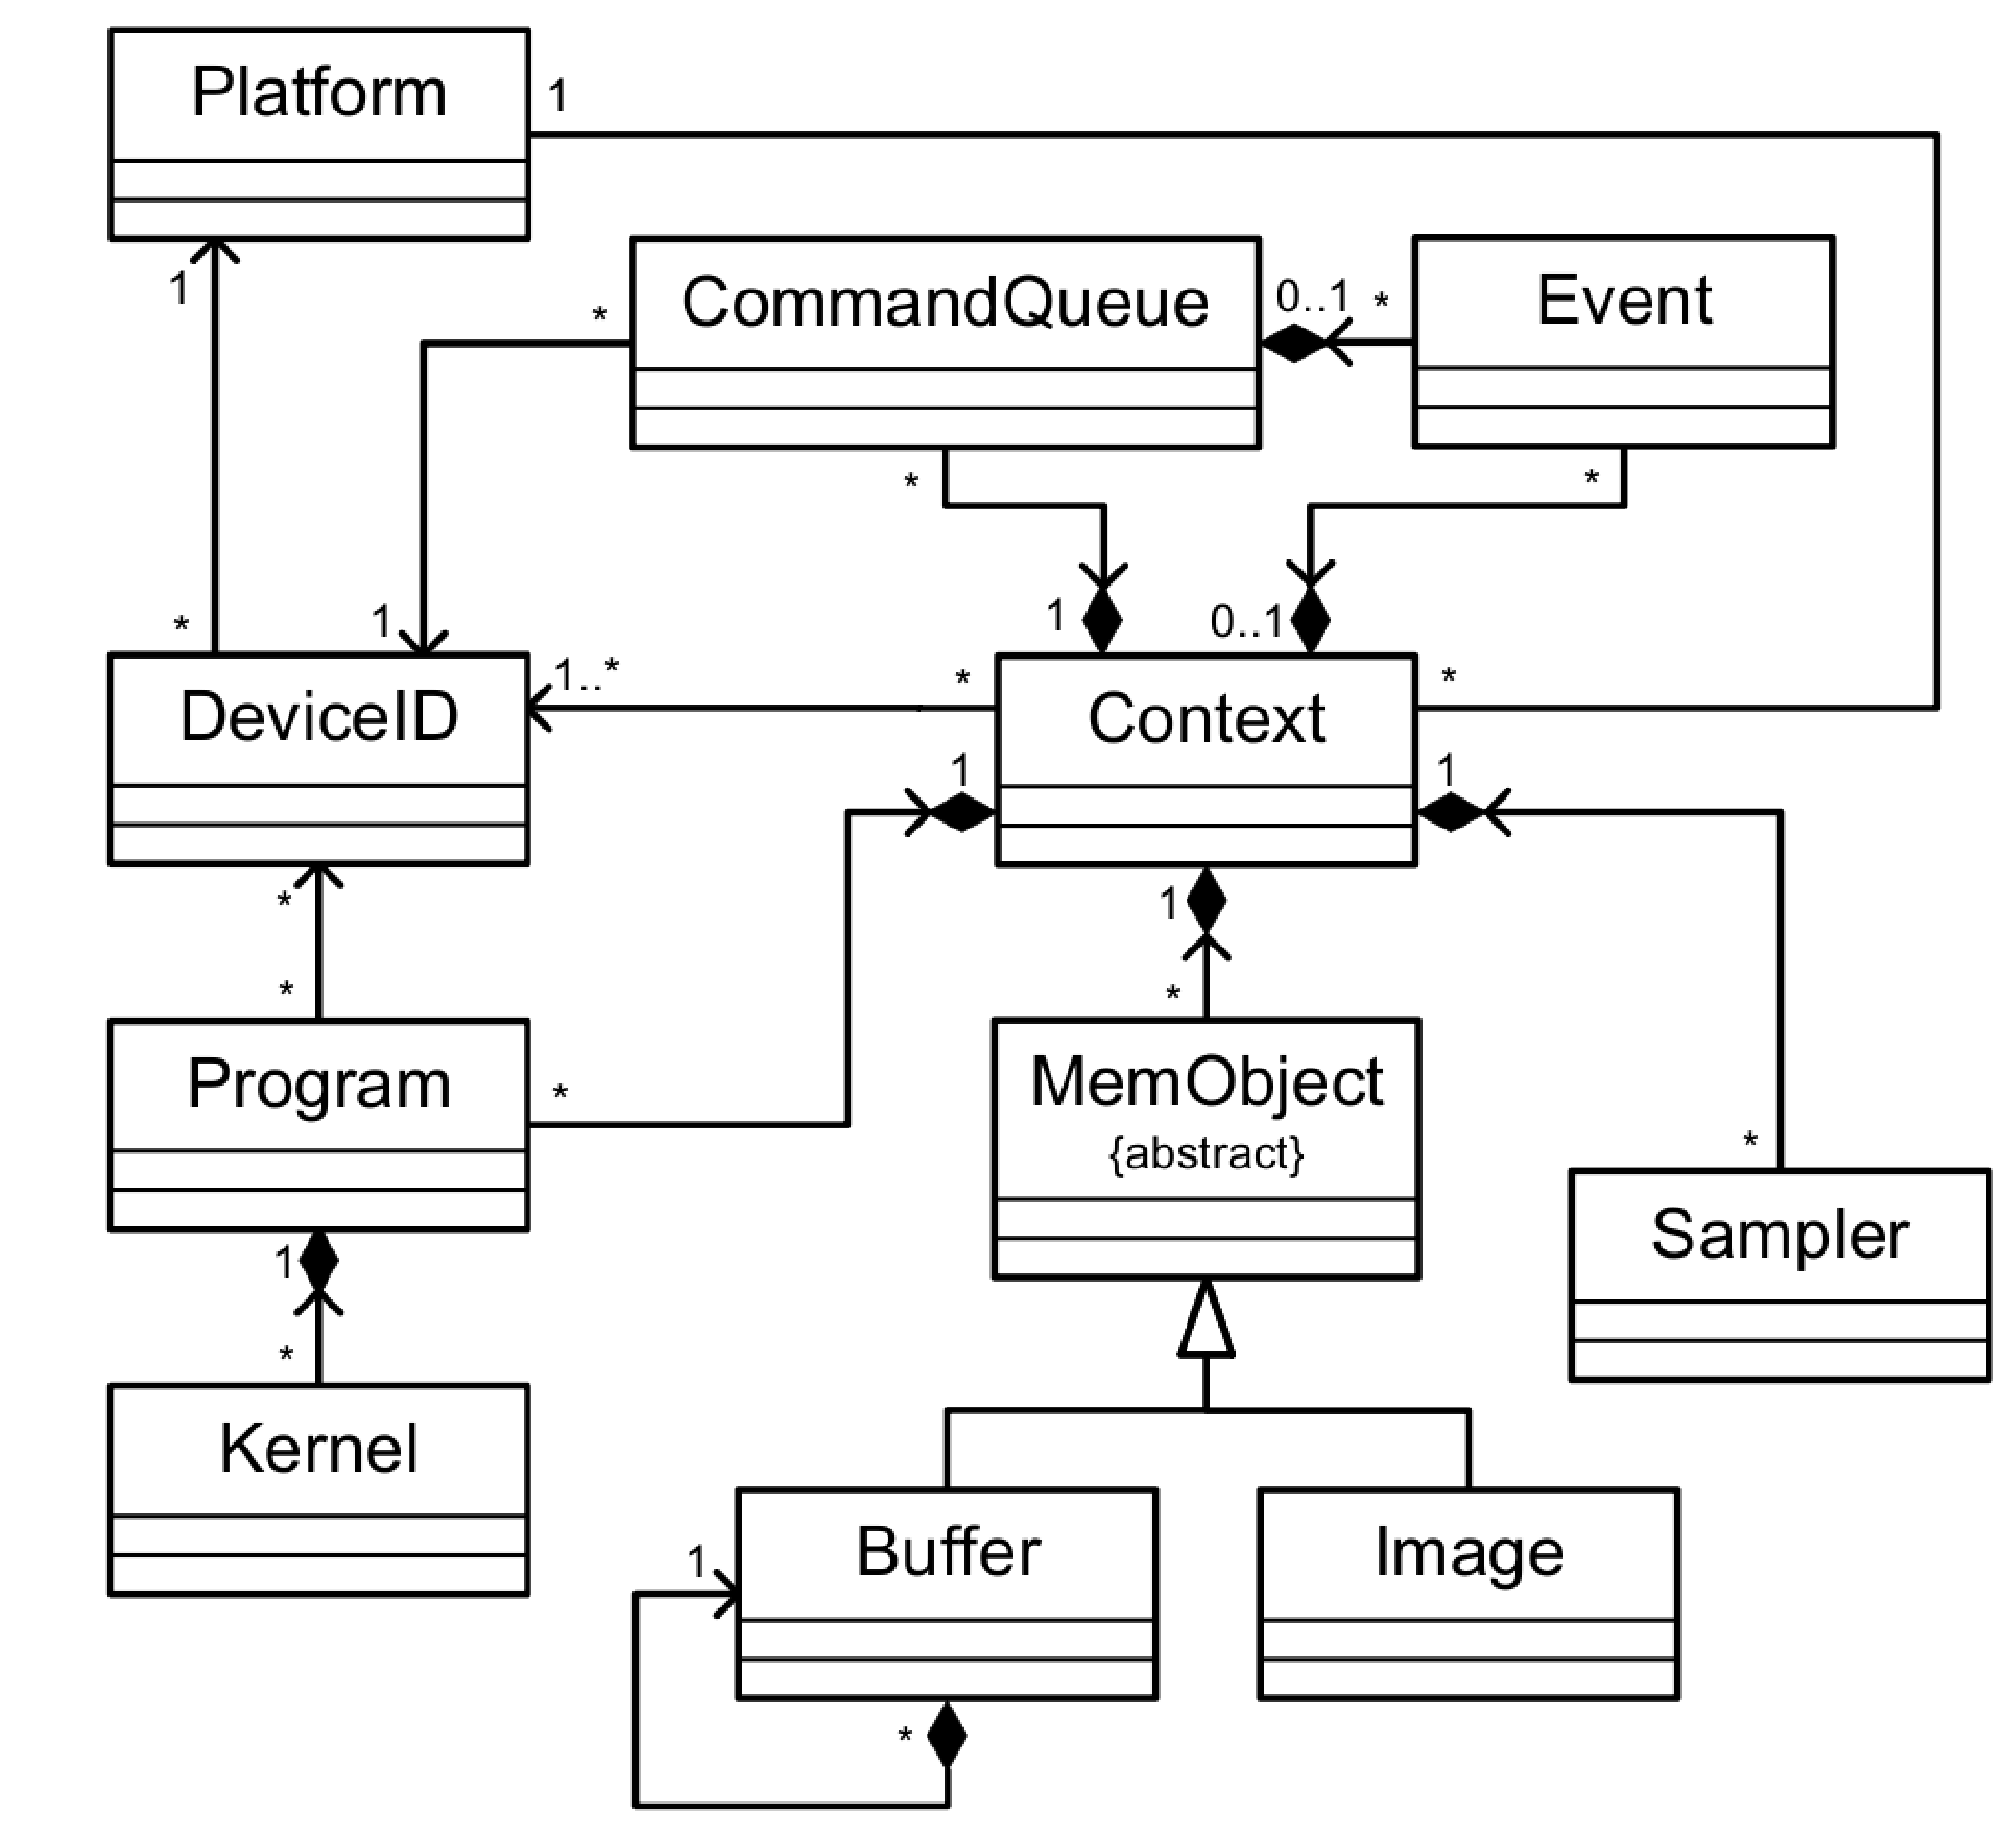
\includegraphics[width=0.6\columnwidth]{figures/eps/context.eps}
		\caption{OpenCL context osztálydiagrammja \cite{opencl}} 
		\label{fig:class} 
	\end{figure}
	Figyelembe kell vennünk azt a megkötést, hogy csak az egy platformon belüli
	eszközök programozhatóak heterogén módon. Például: Intel platform esetén
	lehetséges CPU-t, processzorkártyát és Intel-es GPU-t programozni.
	
	A programozással megoldandó problémát kétféleképpen lehetséges a feldolgozó
	egységekhez (work-item) avagy processzorokhoz rendelni:
	adat parallel módon vagy taszk parallel módon.
	Adat parallel módon (\ref{fig:data_parallel} ábra) a feldolgozandó adat egy
	egységéhez rendelünk egy feldolgozó egységet. Fontos figyelembe venni az eszköz korlátos
	számú feldolgozó egységének számát. Ha nem elég a feldolgozó egysége akkor a
	feladat megfelelő partícionálásával lehetséges kordában tartani a szükséges
	erőforrás számát.
	Taszk parallel módot (\ref{fig:task_parallel} ábra) olyan esetben célszerű
	használna, ha a bemenet dinamikus mérete a futási időben rendkívül változik
	illetve a végrehajtandó feladat lezán függenek össze.
	
	\begin{figure*}[!h]
		\centering
		\subfloat[Adat parallel]{
			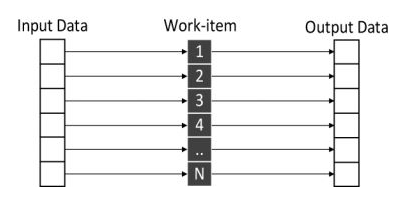
\includegraphics[width=0.45\columnwidth]{figures/eps/data.eps}%
			\label{fig:data_parallel}
		}
		\hfil
		\subfloat[Taszk parallel]{
			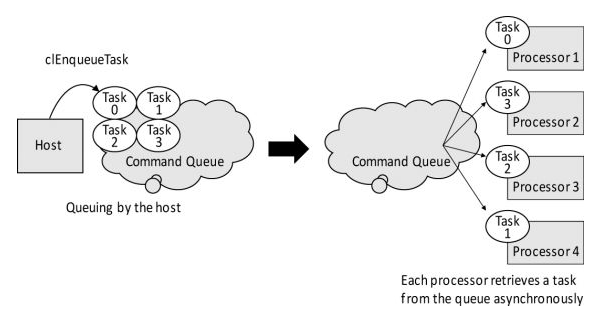
\includegraphics[width=0.45\columnwidth]{figures/eps/task.eps}%
			\label{fig:task_parallel}
		}
		\caption{Feladat hozzárendelése work-item-hez (processzorhoz)}
		\label{fig:parallel}
	\end{figure*}
	A processzor-magok megfelelő kihasználtságának elérése végett több ezer
	work-item virtuális osztozik rajta.
	Továbbá ezen work-item-eket work-group-okba rendezzük, ami a lokális
	memória jogusultsága miatt érdekes.
	Konkrétan egy work-group-ba tartozó összes work-item azonos lokális memórián
	osztozik. Ennek a következménye az, hogy adat parallel módú feldolgozás esetén
	az egymásra ható adatokhoz tartozó work-item-eket egy work groupba kell
	rendelnünk.
	Ha ez nem lehetséges, akkor a globális memóriához kell fordulnunk.
	A globális memória avagy a bank szervezésű külső (off-chip) memóriák
	hozzáférési ideje relatíve nagy így ezek használatát lehetőleg el kell kerülni
	és a programozónak kell ``cahchelni" a lokális memóriába.
	
	
	\begin{center}
	Összefoglalva nagy hangsúlyt kell a memóriaszervezésre fordítani, hogy a
	processzormag megfelelően legyenek az adatokkal táplálva.
	\end{center}


\section{Futási környezet bemutatása}
	
	\begin{table}[!h]
	%\renewcommand{\arraystretch}{1.3}
	% if using array.sty, it might be a good idea to tweak the value of
	% \extrarowheight as needed to properly center the text within the cells
	\caption{Futási környezetek}
	\label{table:envs}
	\centering
	\footnotesize
	% Some packages, such as MDW tools, offer better commands for making tables
	% than the plain LaTeX2e tabular which is used here.
	\begin{tabular}{ l | r | r }
		 & nVidia GT330M & Intel Xeon PHI \\ \hline
		MAX\_COMPUTE\_UNITS & $6$ & $224$\\
		MAX\_WORK\_GROUP\_SIZES & $512\times 512\times 64$ & $8192\times 8192\times 8192$\\
		GLOBAL\_MEM\_SIZE & $1073020928 = 1Gbyte$ & $4514811904 = \sim 4Gbyte$\\
		MAX\_CONSTANT\_BUFFER\_SIZE & $65536$ & $131072$\\
		LOCAL\_MEM\_SIZE & $16384 = 16 Kbyte$ & $32768 = 32 Kbyte$
	\end{tabular}
	\end{table}


\section{Implementációhoz szükséges megfontolások}
	
	A következőkben egy kissebb teljesítményű notebook videókártyát veszek
	alapul a megfontolások demonstrálására. Ez az nVidia GeForce 330M, 
	575 MHz-en futó 48 CUDA core-al, 1024GB memóriával és
	OpenCL 1.0 kompatibilitással.
	A videókártya továbbiakban fontos paraméterei a \ref{table:vcard}. táblázatban
	látható.
	

	
	
	
	Ha a tér ahol a laplace egyenletet meg kell oldanunk nagyon nagy, akkor
	érdemes szétbontani kissebb alterekre és azokhoz rendelni egy-egy
	``work-item''-eket. Mivel a diszkrét laplace egyenlet egy pontja a szomszédos
	pontokkal szoros kapcsolatban van, így az összefüggő ``work-item"-eket egy
	``work-group''-ba érdemes szervezni, mivel így az átlapolódó pontok értékét a
	szomszédos ``work-item'' is tudják írni és olvasni. Az ilyen típusú
	problémának méretét a MAX\_WORK\_GROUP\_SIZES tulajdonság korlátozza.
	
	Jelen esetben a mérési eredmény egy pontjához tartozó tér átlagosan
	$11\times11\times30$ pontból áll.
	Tehát a korábbi nem áll fenn és egyszerű megfeleltetéssel szétoszthatjuk a
	feladatot.
	A teljes tér $512\times512\times11\times11\times30$ méretű, ami $951k$ pont.
	A tárolásához single-precision mellett ennek a számnak a 4-szerese
	szükségeltetik byte-okban mérva. Mivel ez a videókártyán nem áll
	rendelkezésre, így szétbontjuk kissebb feladatrészekre.
	
	Ezen feladatrészek méretét egy paraméter állításával lehet változtati és az
	implementált algoritmus ettől generikusan függ.
	Emellett az interpoláció mértéke is generikusan paraméterrel állítható.
	Az algoritmus generikusságát csupán a futási időben történő dinamikus memória
	allokációval lehetséges megvalósítani. A korábban említettek végett (\ref{table:mem} táblázat)
	az allokáció csak a ``host'' programban történhet.

\section{Memória szervezés}
	\subsection{Csak globális memória használata}
	Az algoritmus pszeudó kódjának direkt leképezése esetén a ``host''-on
	allokálunk memóriát a ``device'' globális memóriájában.
	Majd a megfelelő adatokat ide másoljuk és a kernel is itt ír és olvas.
	A problémát a globális memória nagy hozzáférési ideje jelenti, ami miatt sok
	``work-item'' tétlenül a memóriára fog várakozni.
	Ilyenkor az egy mérési pontra vonatkoztatott szimulációs idő a
	referenciánál is lassabb.
	\subsection{Globális memória és adott esetben lokális memória használata}
	Kis erőfeszítéssel nagy javulást lehet elérni, ha a mérési ponthoz tartozó
	szimulációs tér éppen belefér a lokális memóriába.
	Tehát, mielött az \ref{eq:2} szerinti iteratív megoldót futtatnánk először a
	globális memóriából a lokális memóriába töltjük át a kérdéses pontokat, majd
	számolunk rajt és a végén visszatöltjük a globális memóriába.
	E javítással a referenciával azonos sebességet tudunk elérni.
	\subsection{Globális memória és minden adódó alkalomkor a lokális memória használata}
	Nagyobb erőfeszítést igényel, hogy a globális memórival való kommunikációt a
	lokális memória közbeékelésével tegyünk minden alkalomkor.
	Ezt úgy lehet felfogni, mintha a globális memóriát lokális memória méretű
	kvantumokban tudnám csak elérni.
	Ekkor nagy odafigyelést kíván a memóriacímzés megfelelő prgramozása, de
	eredményképp gyorsulás elérhető. \\
	
	Összegezve elmondható, hogy az aktuálisan használt adat tárolását a lehető
	legközelebb kell tartani a ``compute-unit''-hoz.






